% =====================================================================
% Relatório final (Etapa 3) --- Apresentação e Relatório Final
% Template oficial da SBC (sbc-template.sty e sbc.bst estão nesta pasta).
% Cada pessoa edita SÓ as próprias seções em secoes/ (veja o README.md).
% Compilar: pdflatex etapa3 && bibtex etapa3 && pdflatex etapa3 && pdflatex etapa3
% O enunciado pede de 12 a 15 páginas.
% Antes de entregar, não pode sobrar nenhum \pendente{...} (aparece em vermelho no PDF).
% =====================================================================
\documentclass[12pt]{article}

\usepackage{sbc-template}
\usepackage{graphicx,url}
\usepackage[utf8]{inputenc}
\usepackage[T1]{fontenc}
\usepackage[brazil]{babel}
\usepackage{amsmath,amssymb}
\usepackage{booktabs,tabularx,array}
\usepackage{xcolor}

\newcolumntype{Y}{>{\raggedright\arraybackslash}X}
\graphicspath{{figuras/}}

% Deixa as figuras e tabelas ficarem junto do texto, em vez de sozinhas numa página meio vazia.
\renewcommand{\topfraction}{.85}
\renewcommand{\bottomfraction}{.7}
\renewcommand{\textfraction}{.15}
\renewcommand{\floatpagefraction}{.8}

% Código e nomes de função: \codigo{bfs}
\newcommand{\codigo}[1]{\texttt{#1}}
% Lembrete em vermelho; nenhum pode sobrar na versão entregue.
\newcommand{\pendente}[1]{\textcolor{red}{[PENDENTE: #1]}}

\sloppy

\title{Análise de redes sociais com grafos:\\
       influenciadores na rede da Twitch em português}

% Nomes completos, como no Canvas.
\author{Brunno Enrico Machado Costa\inst{1}, Vitória Rani Santos Menezes\inst{1}, Kaio Ferreira\inst{1},\\
  Iago Verciano Romeiro\inst{1}, Arthur \textcolor{red}{Sobrenome}\inst{1}, Ravi Dornelas e Silva\inst{1}}

\address{\pendente{curso, disciplina e instituição}}

\begin{document}

\maketitle

\begin{abstract}
  This report presents a tool, written in pure Python, that builds, analyzes and visualizes
  social networks modeled as graphs. It reads four real networks and generates synthetic
  graphs; computes degree, paths, centralities (closeness, harmonic, betweenness, PageRank and
  core number), clustering and communities (Louvain and label propagation); simulates SIR
  spreading; and shows the results in a web interface. We apply it to one problem: finding the
  influencers of the network of Twitch streamers who broadcast in Portuguese, and finding which
  centrality ranks them best, by comparing each ranking with the simulated reach and with the
  real number of views. The algorithms were checked against published values and against
  NetworkX, which was used only to compare performance; our centralities ran 1.1 to 9.5 times
  faster than the NetworkX versions we compared with.
  The centralities that measure the position at the center of the network (harmonic, closeness
  and core number) best predict the simulated reach (Kendall $\tau_b$ up to 0.74, against 0.70
  for degree), while PageRank and degree best predict the real views ($\tau_b \approx 0.44$),
  which depend on more than the position in the friendship network.
\end{abstract}

\begin{resumo}
  Este relatório apresenta uma ferramenta, escrita em Python puro, que constrói, analisa e
  visualiza redes sociais modeladas como grafos. Ela lê quatro redes reais e gera grafos
  sintéticos; calcula grau, caminhos, centralidades (proximidade, harmônica, intermediação,
  PageRank e número de núcleo), agrupamento e comunidades (Louvain e propagação de rótulos);
  simula espalhamentos SIR; e mostra os resultados numa interface web. Aplicamos a ferramenta a
  um problema: encontrar os influenciadores da rede de streamers da Twitch que transmitem em
  português e descobrir qual centralidade os ordena melhor, comparando cada ranking com o alcance
  simulado e com as visualizações reais. Os algoritmos foram conferidos com valores publicados e
  com o NetworkX, usado só para comparar o desempenho; nas centralidades, o nosso código foi de
  1,1 a 9,5 vezes mais rápido que as versões do NetworkX comparadas.
  As centralidades que medem a posição no centro da rede (harmônica, proximidade e número de
  núcleo) preveem melhor o alcance simulado ($\tau_b$ de Kendall de até 0,74, contra 0,70 do
  grau), e o PageRank e o grau preveem melhor as visualizações reais ($\tau_b \approx 0{,}44$),
  que dependem de mais do que a posição na rede de amizades.
\end{resumo}

% =====================================================================
% Introdução --- Brunno (Frente 1)
% Só o Brunno edita este arquivo.
% =====================================================================
\section{Introdução}\label{sec:introducao}

Uma rede social pode ser descrita como um grafo: as pessoas são os nós e as relações entre elas,
como amizades ou interações, são as arestas. Com essa representação, perguntas sobre a rede viram
perguntas sobre o grafo. Quem ocupa uma posição central? Que grupos se formam? Quantos passos
separam duas pessoas? Até onde chega uma informação que começa em alguém? A análise de redes
sociais responde a essas perguntas com medidas de grau, caminhos, centralidade, agrupamento e
comunidades~\cite{wasserman1994,newman2018,barabasi2016}. As respostas têm uso prático. Uma
campanha que quer se espalhar depressa procura quem alcança mais gente, e quem tenta conter um
boato precisa saber por onde ele passa.

Encontrar esses espalhadores não é trivial. A escolha mais intuitiva é o grau, ou seja, quem tem
mais amigos. Mas um nó de grau alto na periferia da rede, ligado a nós pouco conectados, espalha
menos que um nó do miolo denso, e simulações de epidemias mostraram que a decomposição em núcleos
($k$-core) acha os melhores espalhadores com mais acerto que o grau~\cite{kitsak2010}. Esses
estudos medem o acerto com o próprio modelo de espalhamento. A rede de streamers da Twitch que
transmitem em português~\cite{rozemberczki2021} permite ir além, porque cada canal traz o número
real de visualizações, uma medida de audiência que não vem do grafo.

Este trabalho desenvolve uma ferramenta que constrói, analisa e visualiza redes sociais e a
aplica a esse problema: identificar os influenciadores da Twitch PT e descobrir qual centralidade
os encontra melhor (Seção~\ref{sec:problema}). Toda a ferramenta foi escrita em Python puro, porque
o enunciado proíbe bibliotecas prontas de grafos, como o NetworkX~\cite{hagberg2008}, que só
aparece na comparação de desempenho. Ela lê quatro redes reais e gera grafos sintéticos; calcula
grau, caminhos mínimos, distâncias, componentes e as centralidades de proximidade, harmônica,
intermediação, PageRank e número de núcleo; mede o agrupamento e detecta comunidades pelos métodos
de Louvain e de propagação de rótulos; simula espalhamentos SIR para comparar o ranking de cada
centralidade com o alcance simulado e com as visualizações reais; e mostra tudo numa interface web,
com o desenho da rede. Cada função tem testes automáticos que comparam o resultado com valores
conhecidos, e o desempenho foi medido em grafos de até 100.000 nós.

O relatório segue esta ordem: trabalhos relacionados (Seção~\ref{sec:trabalhos}), definição do
problema (Seção~\ref{sec:problema}), bases de dados (Seção~\ref{sec:bases}) e modelagem do grafo
(Seção~\ref{sec:modelagem}); os algoritmos e o que eles revelam nas redes
(Seções~\ref{sec:caminhos} a~\ref{sec:comunidades}); a resposta ao problema
(Seção~\ref{sec:influenciadores}); a interface (Seção~\ref{sec:interface}); a avaliação de
desempenho (Seção~\ref{sec:desempenho}); as limitações e os cuidados éticos
(Seção~\ref{sec:limitacoes}); a conclusão (Seção~\ref{sec:conclusao}); e o que cada integrante fez
(Seção~\ref{sec:responsabilidades}).
        % Brunno
% =====================================================================
% Trabalhos relacionados --- Vitória (Frente 2)
% Só a Vitória edita este arquivo.
% =====================================================================
\section{Trabalhos relacionados}\label{sec:trabalhos}

Simulando epidemias SIR em redes reais, um estudo clássico mostrou que o número de núcleo
($k$-core) prevê os melhores espalhadores melhor do que o grau e a intermediação: o que importa é
estar no miolo denso da rede, e não só ter muitos vizinhos~\cite{kitsak2010}. Uma revisão posterior
reuniu dezenas de métodos para encontrar nós importantes, do grau ao PageRank e a métodos de
aprendizado, e os comparou pelo alcance em simulações de espalhamento; nenhuma medida venceu em
todas as redes~\cite{lu2016}. No BraSNAM, grafos de retweets dos protestos brasileiros de 2013
mostraram que o PageRank e a centralidade de autovetor destacam usuários que a simples contagem de
retweets não revela~\cite{theodoro2014}, e, numa rede de pilotos de Fórmula 1, o PageRank deu o
ranking mais informativo entre as centralidades comparadas~\cite{faria2024}.

Este trabalho segue a pergunta do estudo de espalhadores~\cite{kitsak2010}, mas numa rede brasileira, a Twitch em português,
e com dois gabaritos em vez de um: o alcance no SIR e as visualizações reais de cada canal. Além
disso, as seis centralidades comparadas e a simulação foram implementadas do zero, em Python puro,
e conferidas contra valores publicados e contra o NetworkX~\cite{hagberg2008}.         % Vitória
% =====================================================================
% Problema aplicado --- Ravi (Frente 5)
% Só o Ravi edita este arquivo.
% =====================================================================
\section{Problema aplicado}\label{sec:problema}

Queremos saber quais streamers da Twitch PT são os influenciadores e qual centralidade os encontra
melhor. A pergunta se divide em duas: a \textbf{P1} pergunta qual centralidade melhor ordena os
streamers pelo alcance de um espalhamento simulado que começa em cada um, e a \textbf{P2}, qual melhor
os ordena pelas visualizações reais do canal. A hipótese \textbf{H1} é que o número de núcleo supera
o grau na P1, como já se observou em outras redes~\cite{kitsak2010}. A hipótese \textbf{H2} é que
todas as centralidades concordam com as visualizações, mas menos do que com o alcance, porque a
audiência também depende de fatores que o grafo não registra, como a idade do canal.

\paragraph{Entrada e saída.} A entrada é o grafo $G = (V, E)$ da Twitch PT (Seção~\ref{sec:bases}),
com $n = 1.912$ streamers e $m = 31.299$ amizades mútuas, e as visualizações $w(v)$ de cada canal. São
comparadas seis centralidades $c$: grau, proximidade e harmônica (Seção~\ref{sec:caminhos}),
intermediação, PageRank e número de núcleo $k_s$ (Seção~\ref{sec:centralidades}). A saída é o
ranking dos streamers pelo alcance $\rho$, com os empates desfeitos pelo grau e depois pelo
identificador do nó, e, para cada $c$, dois números: $\tau_b(c, \rho)$, a concordância do ranking de
$c$ com o alcance, que responde à P1, e $\tau_b(c, w)$, a concordância com as visualizações, que
responde à P2.

\paragraph{Como validar.} O alcance $\rho(v)$ é a fração média da rede atingida por uma simulação SIR
em tempo discreto que começa só em $v$, repetida $M = 100$ vezes: a cada passo, cada infectado
transmite para cada vizinho suscetível com probabilidade $\beta$ e se recupera no passo seguinte
($\gamma = 1$). Abaixo do limiar epidêmico
$\beta_c = \langle k \rangle / (\langle k^2 \rangle - \langle k \rangle) \approx 0{,}0079$~\cite{newman2002},
todo surto morre pequeno, e muito acima dele quase toda a rede é atingida; nos dois casos, o alcance
não distingue os nós. Por isso, usamos $\beta = 0{,}012 \approx 1{,}5\,\beta_c$, pouco acima do
limiar, como em~\cite{kitsak2010}. A concordância entre uma centralidade $c$ e uma referência
$Y \in \{\rho, w\}$ é o $\tau_b$ de Kendall, a variante que trata os empates~\cite{kendall1945}:
\[
  \tau_b(c, Y) = \frac{P - Q}{\sqrt{(P + Q + T_c)(P + Q + T_Y)}},
\]
em que, entre os $\binom{n}{2}$ pares de nós, $P$ e $Q$ contam os pares concordantes e discordantes,
e $T_c$ e $T_Y$, os empatados só em $c$ ou só em $Y$. O $\tau_b$ só olha a ordem, o que permite
comparar medidas em escalas diferentes, e tratar os empates é essencial, porque o grau assume só 187
valores distintos e $k_s$, só 37. Assim, \textbf{H1}: $\tau_b(k_s, \rho) > \tau_b(\text{grau}, \rho)$;
e \textbf{H2}: $0 < \tau_b(c, w) < \tau_b(c, \rho)$ para toda $c$.
          % Ravi
% =====================================================================
% Bases de dados e grafos sintéticos --- Brunno (Frente 1)
% Só o Brunno edita este arquivo.
% =====================================================================
\section{Bases de dados}\label{sec:bases}

Usamos quatro redes públicas e anonimizadas. As funções de \codigo{leitores/bases.py} leem os
arquivos e descartam laços (arestas de um nó para ele mesmo). As quatro são não direcionadas e conexas, e a
Tabela~\ref{tab:bases} as resume com números calculados pela ferramenta; os testes dos leitores
conferem que os tamanhos lidos são os publicados. Nas três maiores, o grau é muito desigual: a
mediana fica bem abaixo da média, e o maior grau passa de 20 vezes a média na Twitch PT e no
ego-Facebook, uma cauda longa comum em redes sociais~\cite{newman2018}.

\begin{table}[htbp]
\centering
\caption{Bases de dados: $n$ nós, $m$ arestas, densidade $2m/(n(n-1))$ e graus médio, mediano e
máximo, calculados pela ferramenta.}
\label{tab:bases}
\small
\setlength{\tabcolsep}{4.5pt}
\begin{tabular}{@{}l r r r r r r l@{}}
\toprule
Base & $n$ & $m$ & Densidade & \multicolumn{3}{c}{Grau} & Uso \\
\cmidrule(lr){5-7}
 & & & & médio & mediano & máximo & \\
\midrule
Twitch PT & 1.912 & 31.299 & 0,0171 & 32,7 & 17 & 767 & Influenciadores \\
ego-Facebook & 4.039 & 88.234 & 0,0108 & 43,7 & 25 & 1.045 & Desempenho \\
Network of Thrones & 303 & 1.008 & 0,0220 & 6,7 & 4 & 59 & Demonstração \\
Karate Club & 34 & 78 & 0,1390 & 4,6 & 3 & 17 & Corretude \\
\bottomrule
\end{tabular}
\end{table}

A \textbf{Twitch PT} é a rede de amizades mútuas entre streamers que transmitem em português,
coletada por \cite{rozemberczki2021} e distribuída pelo SNAP~\cite{leskovec2014snap}. Cada nó traz
atributos reais: as visualizações do canal, que servem de validação externa para o ranking de
influenciadores, se ele é parceiro da Twitch (279 dos 1.912), se tem conteúdo adulto e há quantos
dias existe. O \textbf{ego-Facebook} une dez redes ego de amizades~\cite{mcauley2012} e, por ser a maior,
serve para medir o desempenho. Na \textbf{Network of
Thrones}, dois personagens do terceiro livro de \emph{As Crônicas de Gelo e Fogo} se ligam quando os
nomes aparecem a até 15 palavras um do outro, e o peso, de 3 a 95, conta quantas vezes isso
acontece~\cite{beveridge2016}; ela serve à demonstração, porque o público reconhece os personagens.
Por fim, o \textbf{Karate Club} é o clube que se dividiu em dois grupos de 17
membros~\cite{zachary1977}, e os seus valores conhecidos servem para provar a corretude.

\paragraph{Grafos sintéticos.} Para testar os algoritmos em tamanhos controlados e medir o
desempenho, \codigo{geradores/modelos.py} gera três modelos clássicos, com uma \codigo{semente} que
repete o grafo. No de \textbf{Erdős--Rényi}~\cite{erdos1959}, cada par de nós se liga com
probabilidade $p$, e o gerador pula direto para o próximo par sorteado, em $O(n + m)$, em vez de
sortear os $n(n-1)/2$ pares~\cite{batagelj2005}. No de \textbf{Barabási--Albert}~\cite{barabasi1999},
cada nó novo se liga a $m$ nós já existentes, com chance proporcional ao grau, o que cria nós muito
conectados, como nas redes reais. No de \textbf{Watts--Strogatz}~\cite{watts1998}, cada nó de um anel
se liga aos $k$ mais próximos e cada aresta é religada com probabilidade $p$, o que mantém o
agrupamento alto e encurta as distâncias. A interface usa os mesmos geradores.
             % Brunno
% =====================================================================
% Modelagem do grafo --- Brunno (Frente 1)
% Só o Brunno edita este arquivo.
% =====================================================================
\section{Modelagem do grafo}\label{sec:modelagem}

Cada rede vira um grafo simples $G = (V, E)$, com $n = |V|$ nós e $m = |E|$ arestas. Na Twitch PT,
cada nó é um streamer e cada aresta, uma amizade mútua, sem peso; na Network of Thrones, o peso
$w(e)$ é o número de interações entre os dois personagens; nas redes sem peso, $w(e) = 1$.

\paragraph{Estrutura.} As redes sociais são esparsas: na Twitch PT, só 1,7\% dos pares possíveis
são amizades. Uma matriz de adjacência guardaria $n^2 = 3{,}66$ milhões de células, 98\% delas com
zero, e a busca em largura, base de quase todos os algoritmos do trabalho, custaria $\Theta(n^2)$; a
lista de adjacência guarda só as arestas que existem, em $O(n + m)$, e faz a mesma busca em
$\Theta(n + m)$~\cite{cormen2022}. A classe \codigo{Grafo} guarda essa lista como um dicionário de
dicionários, em que \codigo{\_adj[v][w]} é o peso da aresta entre $v$ e $w$. Assim, inserir um nó,
inserir ou remover uma aresta, testar se ela existe e ler o peso e o grau custam $O(1)$ em
média~\cite{pythoncomplexidade}; percorrer os vizinhos de $v$ custa $O(\text{grau}(v))$, e contar os
nós e as arestas, $O(1)$, porque $m$ é atualizado a cada inserção e remoção. O peso fica junto do
vizinho, o que atende a Network of Thrones e o Louvain, que cria arestas com peso ao agrupar
comunidades, e os nós podem ser de qualquer tipo imutável, como números na Twitch PT e nomes na
Network of Thrones. O NetworkX adota a mesma estrutura pelos mesmos motivos~\cite{hagberg2008}.

\paragraph{Outras decisões.} No grafo direcionado, a classe guarda à parte os predecessores de cada
nó (\codigo{\_pred}), para o grau de entrada e o PageRank~\cite{brin1998}; no não direcionado,
\codigo{\_pred} é o próprio \codigo{\_adj}, sem cópia. Os laços, que o Louvain cria ao agrupar
comunidades, contam duas vezes no grau, para a soma dos graus ser sempre $2m$. Nos algoritmos mais
pesados, o \codigo{IndexadorDeNos} renumera os nós de $0$ a $n-1$, e a adjacência vira uma lista de
listas, que o Python percorre mais depressa que dicionários.

\paragraph{Diagramas.} A Figura~\ref{fig:uml} mostra o núcleo e os pacotes. Os demais pacotes são
módulos de funções que recebem um \codigo{Grafo}, não o alteram e devolvem um valor por nó
(\codigo{dict[nó, valor]}), um contrato comum a todo o grupo; os leitores e os geradores criam
grafos, a interface só chama as funções, e o NetworkX aparece apenas em \codigo{desempenho/}. A
Figura~\ref{fig:uml-comportamento} traz os diagramas comportamentais da Etapa 1, que estão em tamanho
real em \codigo{documentos/uml/}.

\begin{figure}[htbp]
\centering
\begin{minipage}[b]{.52\textwidth}
  \centering
  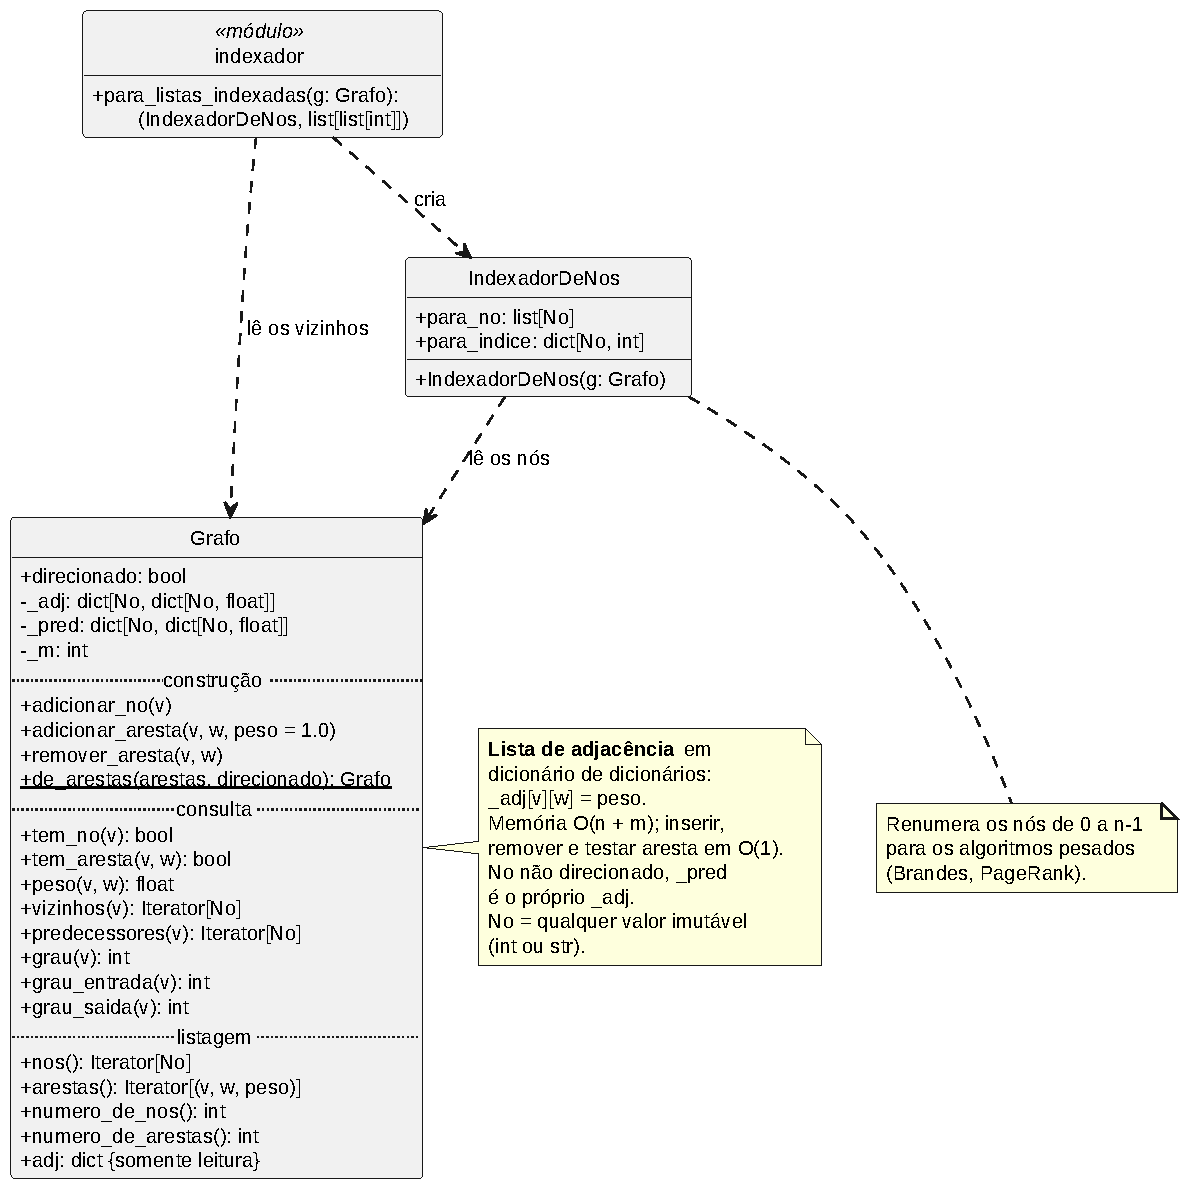
\includegraphics[width=\textwidth]{classes.pdf}\\[2pt]
  {\small (a) Classes do núcleo (\codigo{redes/nucleo})}
\end{minipage}\hfill
\begin{minipage}[b]{.36\textwidth}
  \centering
  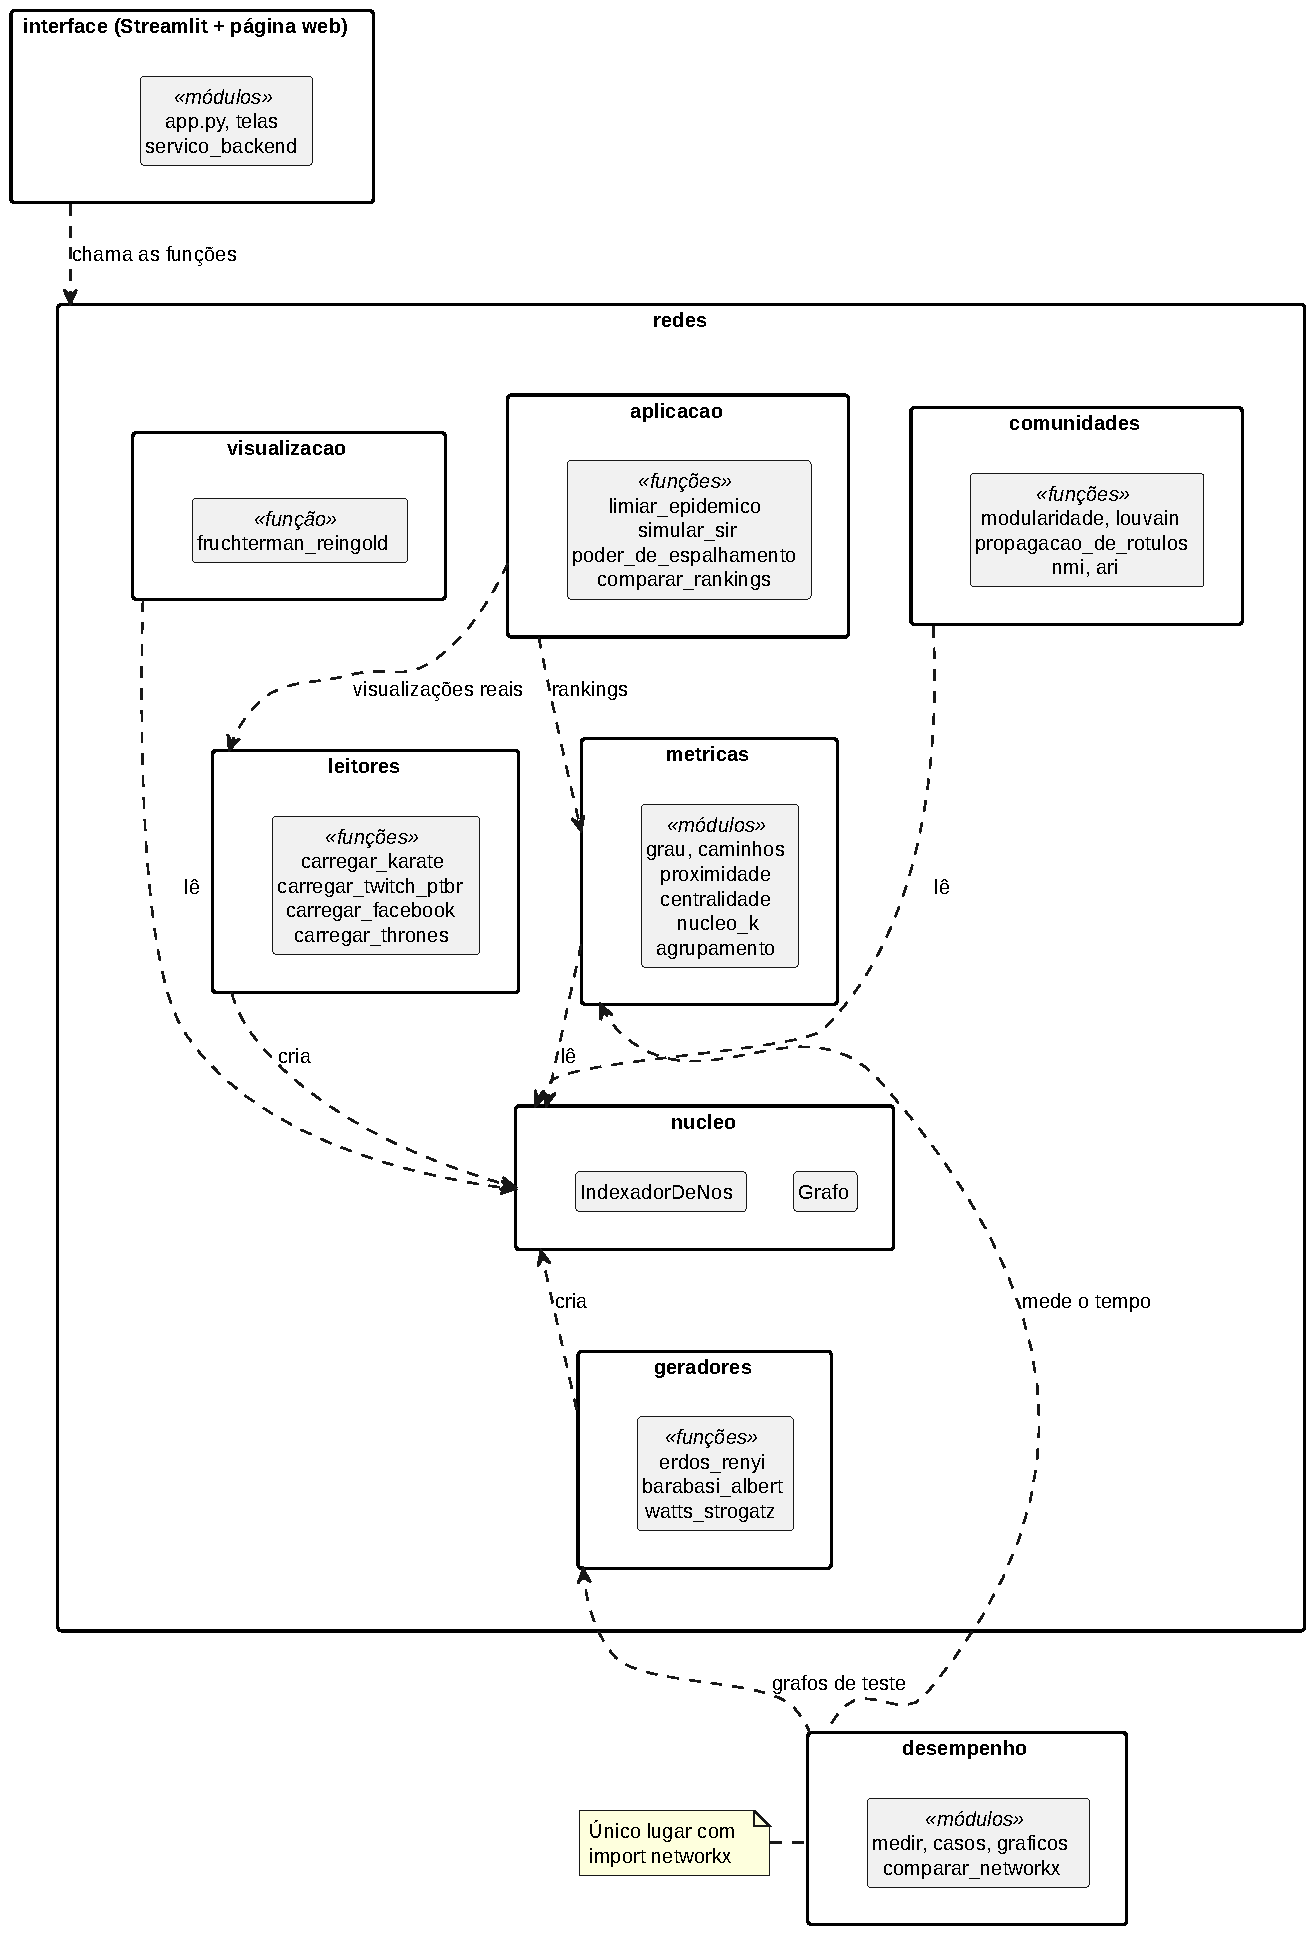
\includegraphics[width=\textwidth]{pacotes.pdf}\\[2pt]
  {\small (b) Pacotes}
\end{minipage}
\caption{Diagramas UML da estrutura do código. Em (b), as setas tracejadas indicam dependência:
quem aponta usa o pacote apontado.}
\label{fig:uml}
\end{figure}

\begin{figure}[htbp]
\centering
\begin{minipage}[b]{.38\textwidth}
  \centering
  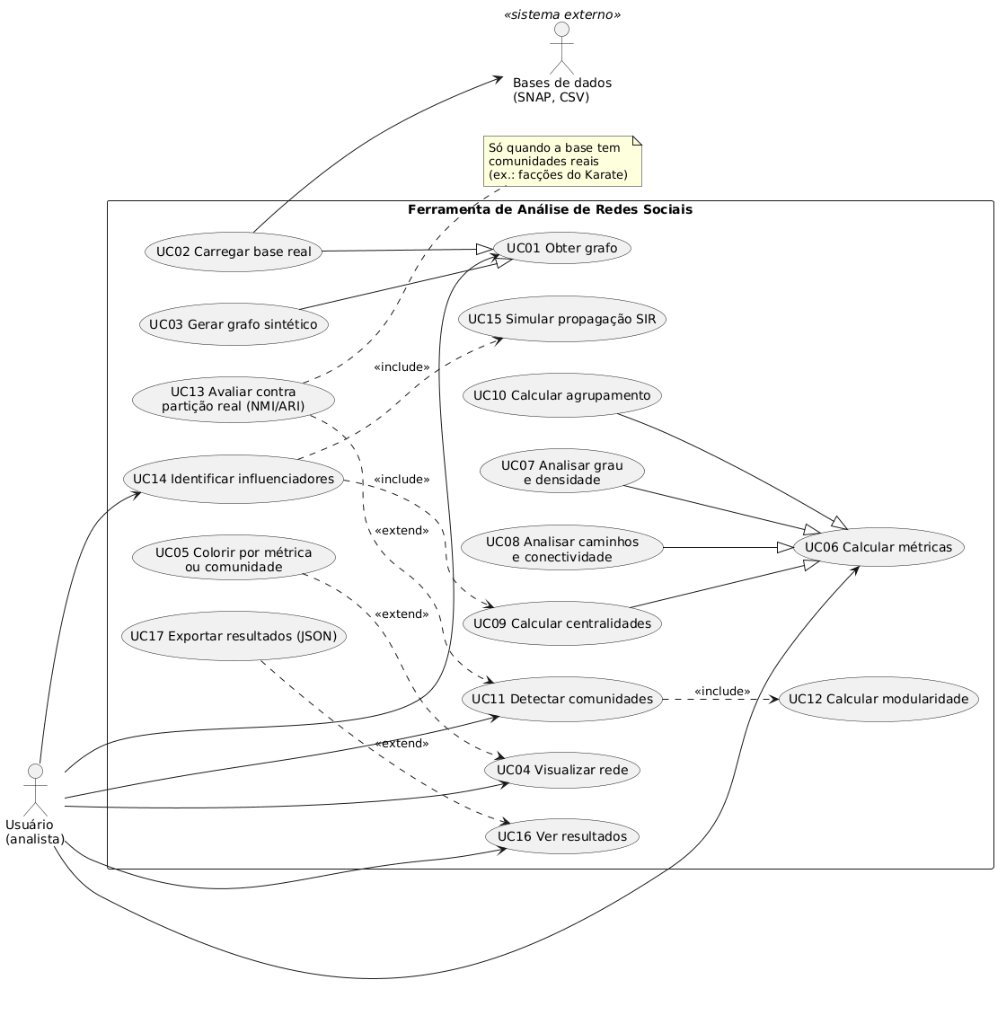
\includegraphics[width=\textwidth]{casos_de_uso.jpg}\\[2pt]
  {\small (a) Casos de uso}
\end{minipage}\hfill
\begin{minipage}[b]{.33\textwidth}
  \centering
  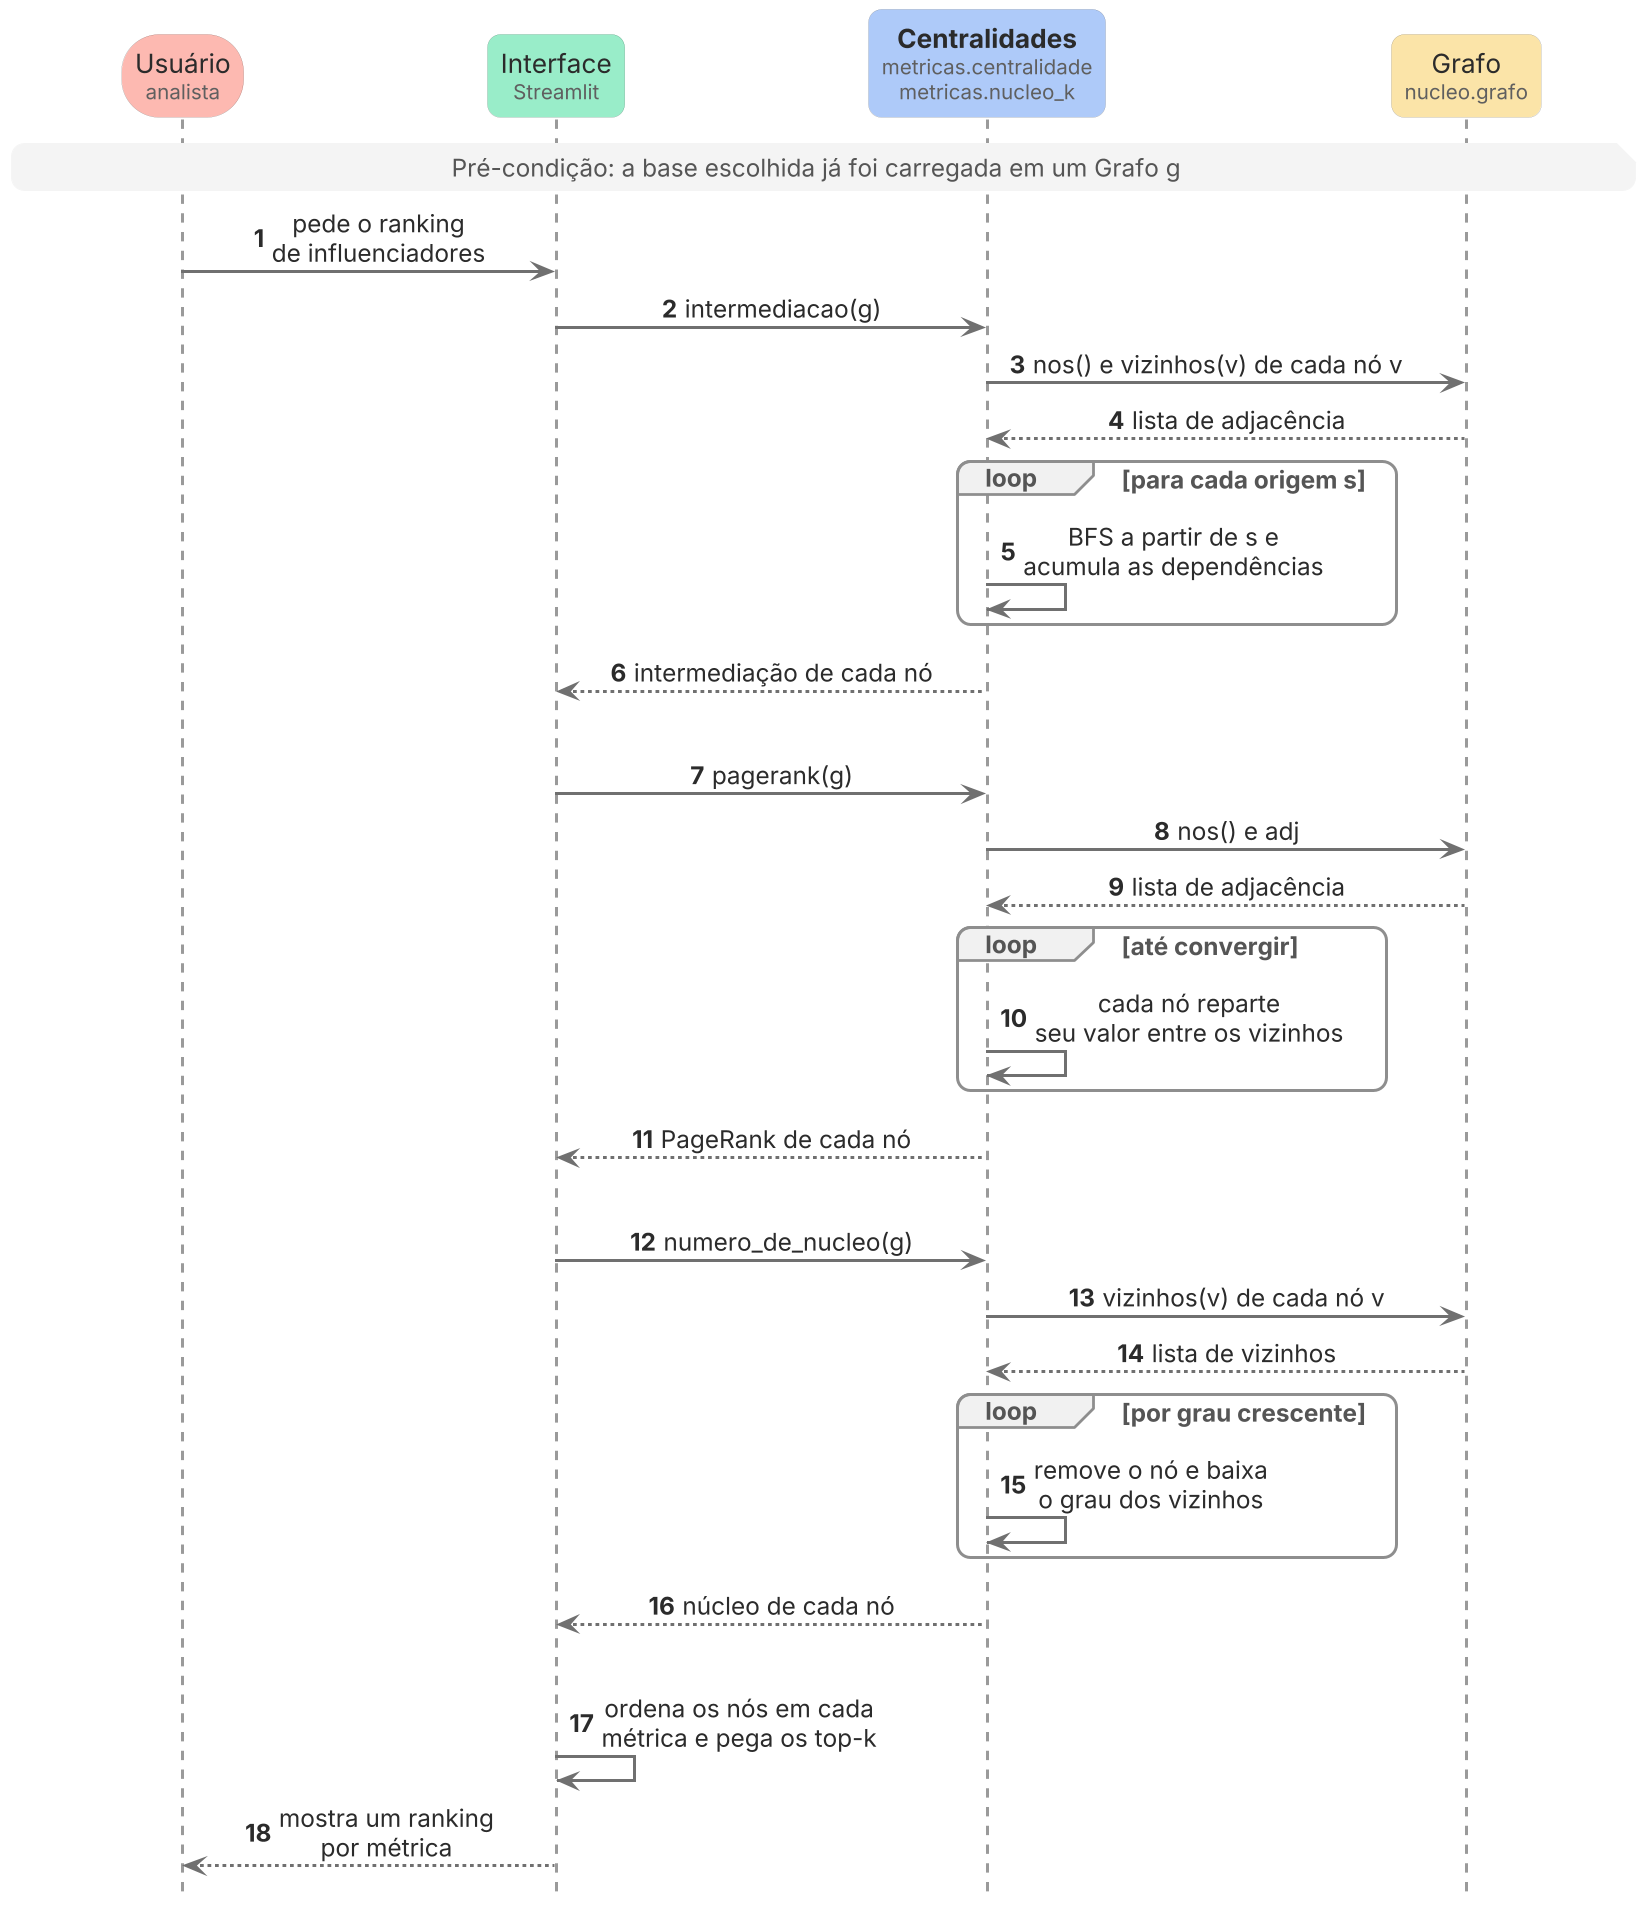
\includegraphics[width=\textwidth]{sequencia.png}\\[2pt]
  {\small (b) Sequência do ranking}
\end{minipage}\hfill
\begin{minipage}[b]{.21\textwidth}
  \centering
  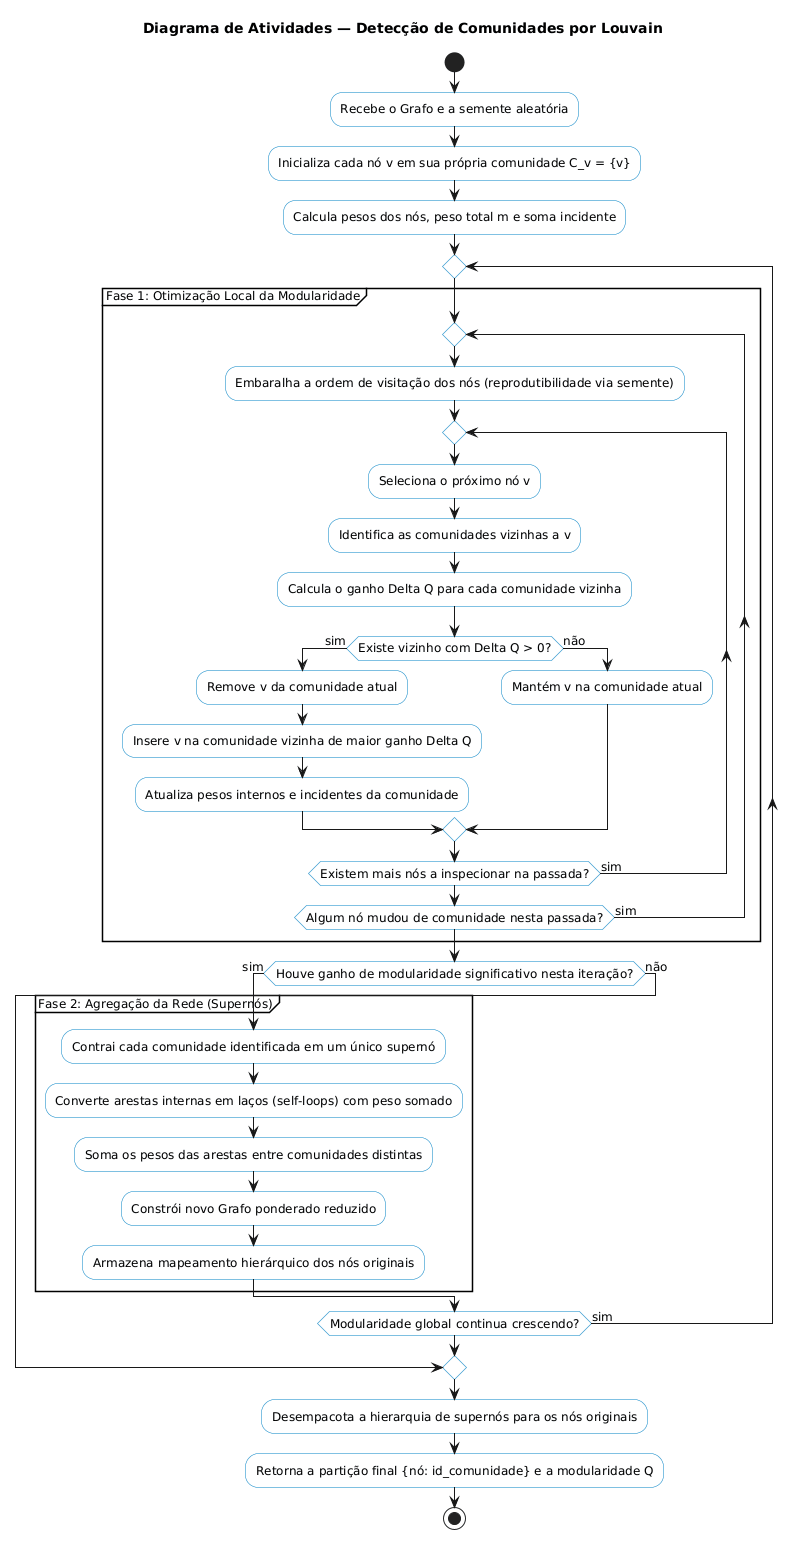
\includegraphics[width=\textwidth]{atividades_louvain.png}\\[2pt]
  {\small (c) Atividades do Louvain}
\end{minipage}
\caption{Diagramas comportamentais da Etapa 1: (a) os 17 casos de uso da ferramenta; (b) as chamadas
que montam o ranking de influenciadores; (c) as duas fases do método de Louvain.}
\label{fig:uml-comportamento}
\end{figure}

\paragraph{Corretude.} A classe, os leitores e os geradores têm 41 testes (\codigo{pytest}): grafos
de resposta conhecida, como o completo $K_5$; propriedades conferidas pelo \codigo{Hypothesis} em
centenas de grafos aleatórios, como a soma dos graus ser $2m$; os tamanhos das quatro bases; e o
número de arestas de cada gerador.
         % Brunno
% =====================================================================
% Grau, caminhos e proximidade --- Vitória (Frente 2)
% Só a Vitória edita este arquivo. Apague o \pendente quando escrever a seção.
% =====================================================================
\section{Grau, caminhos e proximidade}\label{sec:caminhos}

\pendente{Vitória: o que cada função calcula (grau, densidade, BFS, DFS, componentes, Dijkstra, distância média, diâmetro, proximidade e harmônica), a complexidade, como foi validada (testes e valores de referência) e o que os números mostram nas bases (por exemplo, na Twitch PT, distância média de 2,53 e diâmetro 7). Até 3/4 de página.}
          % Vitória
% =====================================================================
% Centralidades --- Iago (Frente 3)
% Só o Iago edita este arquivo.
% =====================================================================
\section{Centralidades}\label{sec:centralidades}

Além do grau e da proximidade, a ferramenta calcula três centralidades: a intermediação, que mede
quanto o nó serve de ponte entre os outros; o PageRank, que mede o prestígio de receber ligações de
nós também importantes; e o número de núcleo ($k$-core), que diz se o nó está no miolo mais denso
da rede. As funções, em \codigo{metricas/centralidade.py} e \codigo{metricas/nucleo\_k.py}, recebem
um \codigo{Grafo} sem alterá-lo, devolvem um valor por nó e, nos laços mais pesados, trocam os nós
por inteiros de $0$ a $n-1$ e as adjacências por listas, que o Python percorre mais depressa que
dicionários.

\paragraph{Intermediação.} A intermediação de $v$ soma, sobre os pares $s \neq v \neq t$, a fração
dos caminhos mínimos de $s$ a $t$ que passam por $v$:
\[
  C_B(v) = \sum_{s \neq v \neq t} \frac{\sigma_{st}(v)}{\sigma_{st}},
\]
em que $\sigma_{st}$ é o número de caminhos mínimos de $s$ a $t$ e $\sigma_{st}(v)$, o número dos
que passam por $v$. Calcular todos os pares e depois somar custaria $O(n^3)$. O algoritmo de
Brandes~\cite{brandes2001} faz uma busca em largura a partir de cada origem $s$, contando os
caminhos mínimos, e depois percorre os nós do mais distante para o mais próximo, acumulando
\[
  \delta_s(v) = \sum_{w \,:\, v \in P_s(w)} \frac{\sigma_{sv}}{\sigma_{sw}} \bigl(1 + \delta_s(w)\bigr),
\]
em que $P_s(w)$ são os nós que vêm logo antes de $w$ nos caminhos mínimos a partir de $s$. A soma
de $\delta_s(v)$ sobre todas as origens dá a intermediação de $v$, em tempo $O(nm)$ e espaço
$O(n + m)$, e o resultado é dividido por $(n-1)(n-2)$, como no NetworkX~\cite{hagberg2008}. Nas
redes grandes, a função pode usar só $k$ origens sorteadas e multiplicar a soma por $n/k$, uma
estimativa sem viés da versão exata~\cite{brandes2007}, em tempo $O(km)$.

\paragraph{PageRank.} O PageRank~\cite{brin1998} modela um navegador aleatório que, a cada passo,
segue uma aresta de saída com probabilidade $d = 0{,}85$, escolhida em proporção ao peso, ou salta
para um nó qualquer com probabilidade $1 - d$. O PageRank de um nó é a fração do tempo que o
navegador passa nele, calculada por iteração de potência:
\[
  x^{(t+1)}_j = \frac{1 - d}{n} + d \sum_{i \to j} \frac{w_{ij}}{w_i}\, x^{(t)}_i
               + \frac{d}{n} \sum_{i \in D} x^{(t)}_i ,
\]
em que $w_i$ é o peso total que sai de $i$ e $D$ é o conjunto dos nós sem saída, cujo valor é
repartido entre todos. Cada iteração custa $O(n + m)$, e o laço para quando a soma das diferenças
entre duas iterações fica abaixo de $n \cdot 10^{-8}$, o critério do NetworkX; na Twitch PT, isso
leva 18 iterações. Se o limite de 100 iterações for atingido, o que pode acontecer em grafos
bipartidos, a função emite um aviso em vez de falhar.

\paragraph{Núcleos.} O $k$-núcleo é o maior subgrafo em que todo nó tem pelo menos $k$ vizinhos
dentro dele, e o número de núcleo de $v$ é o maior $k$ cujo $k$-núcleo contém $v$; os nós de núcleo
alto costumam ser bons espalhadores~\cite{kitsak2010}. O algoritmo de Batagelj e
Zaversnik~\cite{batagelj2003} remove sempre o nó de menor grau que restou: o grau dele nesse
momento é o seu número de núcleo, e cada remoção diminui em 1 o grau dos vizinhos. Com os nós em
baldes por grau, cada aresta é tratada uma única vez, em tempo total $O(n + m)$.

\paragraph{Validação.} As funções têm 42 testes (\codigo{pytest} e \codigo{Hypothesis}), com casos
de resposta conhecida (estrela, grafo completo, caminho, ciclo, grafos desconexos e direcionados),
invariantes em grafos aleatórios e valores de referência calculados com o NetworkX 3.7. Todos
conferem: no Karate Club, por exemplo, a intermediação dos nós 0, 33 e 32 é 0,4376, 0,3041 e
0,1452, e o núcleo máximo é 4; na Twitch PT, o nó 127 tem a maior intermediação (0,0993) e o maior
PageRank (0,0119), e o núcleo máximo é 37, com 154 nós. Nas medições da
Seção~\ref{sec:desempenho}, os resultados também foram comparados nó a nó com os do NetworkX nos 25
grafos medidos, com diferença máxima de $5{,}6 \cdot 10^{-17}$, ou seja, só arredondamento.

\paragraph{O que as métricas mostram.} Na Twitch PT, as três concordam no topo: os cinco maiores
valores de intermediação e de PageRank são dos mesmos cinco streamers (nós 127, 1476, 1297, 290 e
467), 8 dos 10 primeiros coincidem nas duas listas, e todos eles estão no núcleo 37, o miolo de 154
nós (8\% da rede) em que cada um tem pelo menos 37 amigos dentro do próprio miolo. Na Network of
Thrones, ao contrário, elas discordam: Tyrion Lannister tem o maior grau, e Jon Snow, a maior
intermediação e o maior PageRank com peso (o número de vezes que dois personagens aparecem juntos);
sem o peso, o PageRank põe Tyrion à frente. Cada métrica capta um aspecto diferente da importância
de um nó, e por isso o ranking de influenciadores compara todas elas com o alcance no espalhamento
SIR.
     % Iago
% =====================================================================
% Agrupamento e comunidades --- Arthur (Frente 4)
% Só o Arthur edita este arquivo. Apague o \pendente quando escrever a seção.
% =====================================================================
\section{Agrupamento e comunidades}\label{sec:comunidades}

\pendente{Arthur: triângulos, agrupamento e transitividade; modularidade; Louvain, com o diagrama de atividades; propagação de rótulos; NMI e ARI. Complexidade, validação (Karate: agrupamento médio 0,5706 e $Q \approx 0{,}42$; Twitch PT: $Q$ entre 0,286 e 0,296) e o que as comunidades mostram. Até 1 página.}
       % Arthur
% =====================================================================
% Influenciadores: resultados do problema aplicado --- Ravi (Frente 5)
% Só o Ravi edita este arquivo.
% =====================================================================
\section{Influenciadores na Twitch PT}\label{sec:influenciadores}

As funções ficam em \codigo{aplicacao/influencia.py}, e \codigo{aplicacao/experimento.py} roda o
experimento e grava os resultados em \codigo{aplicacao/resultados/}. A tela de influenciadores
(Seção~\ref{sec:interface}) usa as mesmas funções e os mesmos parâmetros.

\paragraph{Limiar e simulação.} A função \codigo{limiar\_epidemico} calcula $\beta_c$ a partir dos
graus, em $O(n)$. A função \codigo{simular\_sir} faz uma rodada: a cada passo, cada infectado tenta
transmitir uma vez para cada vizinho suscetível e se recupera. Os estados ficam num vetor de bytes
que só é limpo nos nós atingidos, então cada rodada custa o tamanho do surto, e $O(n + m)$ no pior
caso. A função \codigo{poder\_de\_espalhamento} repete a rodada $M = 100$ vezes a partir de cada
nó, em $O(M n (n + m))$ no pior caso. Perto do limiar, quase todos os surtos são pequenos, e as
191.200 rodadas levam cerca de 15\,s. Com $\beta = 0{,}012$ e semente 2026, os atingidos por rodada
vão de 1 a 88 (4,6\% da rede), com mediana de 7,4.

\paragraph{Concordância.} A função \codigo{tau\_de\_kendall} calcula o $\tau_b$ pelo algoritmo de
Knight~\cite{knight1966}, na versão com empates~\cite{christensen2005}. Ela ordena os pares
$(c(v), Y(v))$ e conta os pares discordantes como inversões num merge sort, em $O(n \log n)$. Na
Twitch PT, isso leva 4\,ms, contra 0,7\,s para comparar os 1,8 milhão de pares um a um. A função
\codigo{comparar\_rankings} aplica o $\tau_b$ a cada par de centralidade e referência.

\paragraph{Validação.} As funções têm 66 testes (\codigo{pytest} e \codigo{Hypothesis}). O limiar dá
o valor exato no grafo completo, $1/(n-2)$, na estrela, $2/(n-2)$, e no ciclo, 1. Com $\beta = 0$,
o SIR atinge só a origem, e com $\beta = 1$, a componente inteira. O alcance médio coincide, a menos
de 0,01, com o valor calculado à mão, por exemplo $(1+\beta)/2$ numa aresta. O $\tau_b$ dá 1 e $-1$
em rankings iguais e invertidos, dá $5/\sqrt{30}$ num caso com empate e coincide com a contagem par
a par em 200 casos aleatórios. Na Twitch PT, o $\tau_b$ do grau, do PageRank e do núcleo contra as
visualizações bate com os valores de referência obtidos com o NetworkX (0,43, 0,44 e 0,40).

\begin{table}[htbp]
\centering
\caption{$\tau_b$ de Kendall entre o ranking de cada centralidade e as duas referências, na Twitch
PT ($\beta = 0{,}012$, $\gamma = 1$, 100 rodadas por nó, semente 2026).}
\label{tab:concordancia}
\small
\begin{tabular}{@{}l r r@{}}
\toprule
Centralidade & $\tau_b$ com o alcance (P1) & $\tau_b$ com as visualizações (P2) \\
\midrule
Grau & 0,7033 & 0,4326 \\
Proximidade & 0,7344 & 0,2889 \\
Harmônica & \textbf{0,7435} & 0,3031 \\
Intermediação & 0,5341 & 0,4133 \\
PageRank & 0,6592 & \textbf{0,4386} \\
Número de núcleo & 0,7301 & 0,4034 \\
\bottomrule
\end{tabular}
\end{table}

\paragraph{Resultados.} A Tabela~\ref{tab:concordancia} responde às duas perguntas. Na \textbf{P1},
as centralidades que medem a posição no centro da rede ficam à frente: a harmônica (0,7435), a
proximidade e o núcleo. A intermediação fica em último (0,5341), porque ser ponte entre grupos não
faz de um nó um bom ponto de partida. Com as sementes 1, 2 e 3, a ordem das seis se repete. Com
$\beta = 0{,}016$ ($2\beta_c$), o núcleo passa à frente da harmônica. A \textbf{H1} se confirma: o
núcleo supera o grau (0,7301 contra 0,7033), também nessas variações. Na \textbf{P2}, o PageRank
(0,4386) e o grau (0,4326) preveem melhor as visualizações, e a proximidade e a harmônica, as
melhores na P1, são as piores. A \textbf{H2} também se confirma: todas as centralidades concordam
com as visualizações, mas menos do que com o alcance. O próprio alcance concorda com as
visualizações só com $\tau_b = 0{,}3376$, o que indica que a audiência depende de fatores que a rede
de amizades não registra.
   % Ravi
% =====================================================================
% Interface --- Kaio (Frente 6)
% Só o Kaio edita este arquivo. Apague o \pendente quando escrever a seção.
% =====================================================================
\section{Interface}\label{sec:interface}

\pendente{Kaio: como a interface funciona (Streamlit, servidor local e as seis telas), o posicionamento de Fruchterman--Reingold (complexidade e a versão rápida acima de 400 nós) e dois ou três prints das telas em figuras/. Até 1 página.}
         % Kaio
% =====================================================================
% Avaliação de desempenho --- Iago (Frente 3)
% Só o Iago edita este arquivo. Os números vêm de desempenho/resultados/.
% =====================================================================
\section{Avaliação de desempenho}\label{sec:desempenho}

Para verificar se as complexidades se confirmam na prática e quanto custa o Python puro, medimos as
centralidades da Seção~\ref{sec:centralidades} e a busca em largura (BFS) com o nosso código e com o
NetworkX 3.7~\cite{hagberg2008}, que o enunciado só permite usar nesta comparação. Os scripts e os
resultados completos ficam em \codigo{desempenho/}.

\paragraph{Metodologia.} Usamos grafos de Erdős--Rényi, Barabási--Albert e Watts--Strogatz
($p = 0{,}1$) com 1.000 a 100.000 nós, grau médio 10 e semente 42, além das quatro bases. O tempo é a
mediana de 5 execuções com \codigo{time.perf\_counter}, e o pico de memória é o que a função aloca
durante a chamada, medido com \codigo{tracemalloc}; na BFS, medimos também as arestas percorridas por
segundo (TEPS). No NetworkX, o PageRank é a versão em Python puro, porque a padrão depende do SciPy.
A intermediação exata, de custo $O(nm)$, só foi medida até 5.000 nós, em que já leva cerca de
20~s; acima disso, só a amostrada, com $k = 100$. As medições rodaram num AMD Ryzen 5 7600X com
14,7~GiB de RAM, Ubuntu 24.04 e Python 3.12.3.

\begin{figure}[tb]
\centering
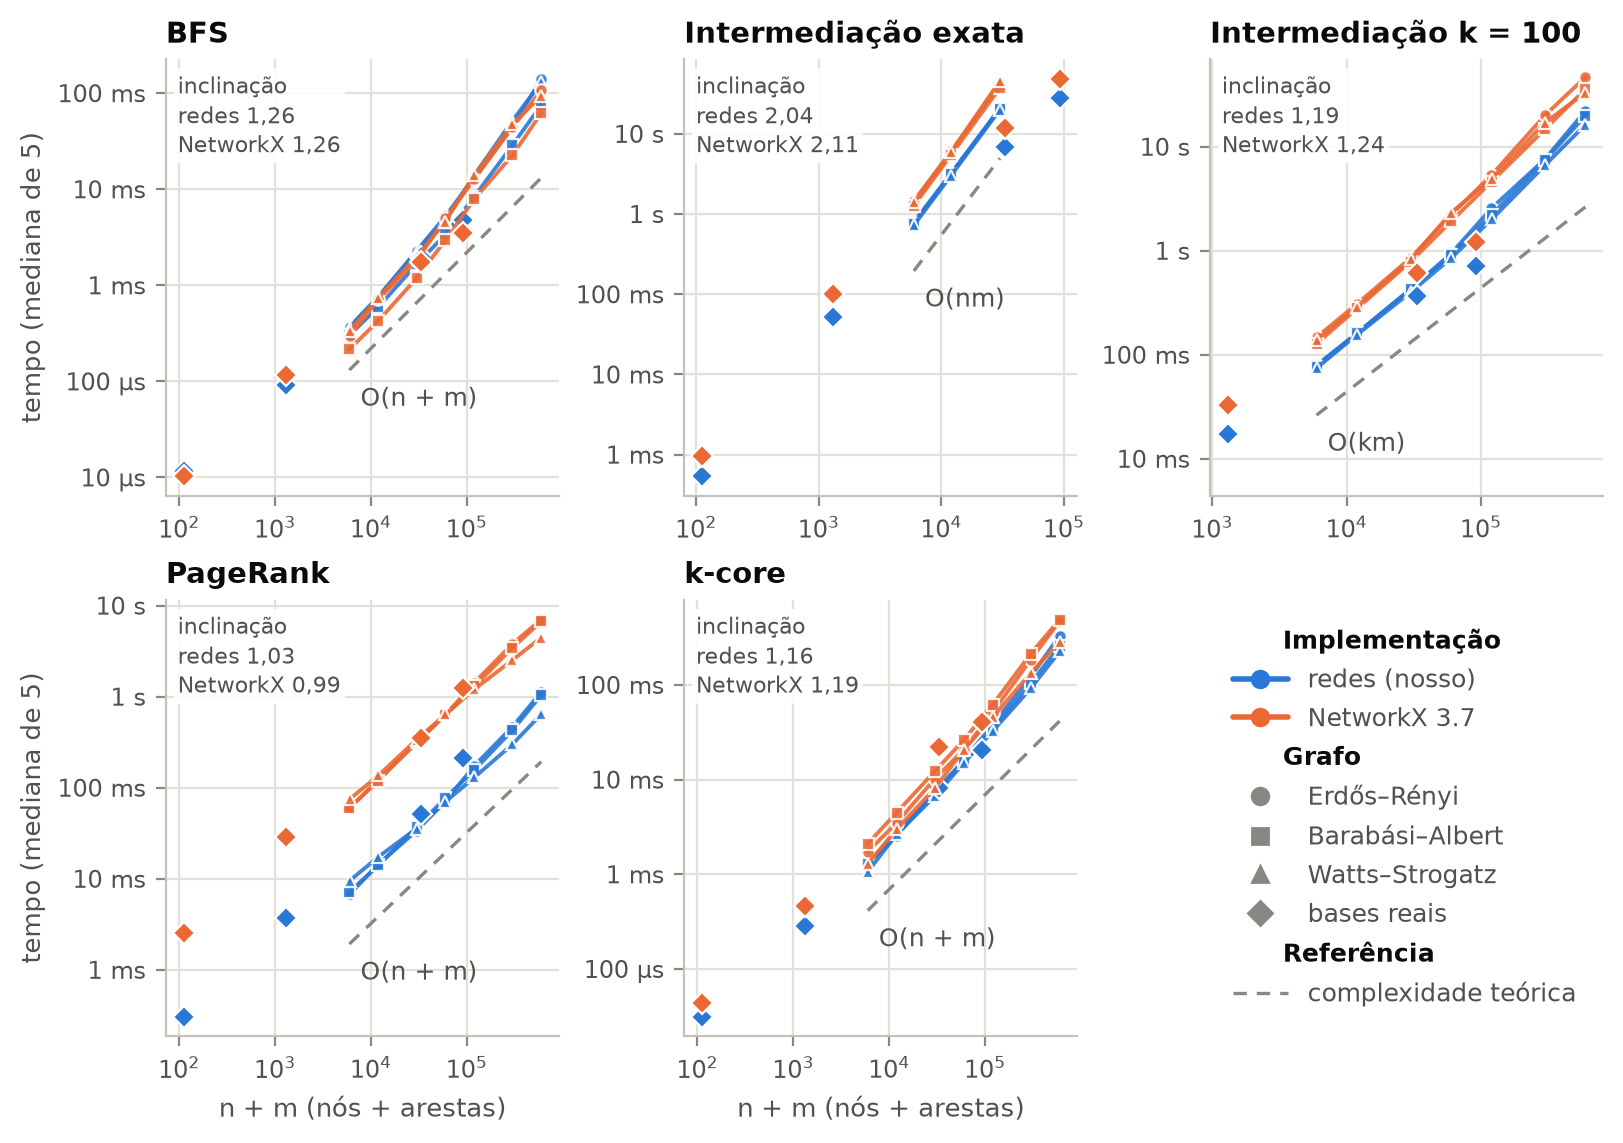
\includegraphics[width=.7\textwidth]{tempo_loglog.png}
\caption{Tempo (mediana de 5 execuções) em função de $n + m$, em escala log-log. Azul: nosso
código; laranja: NetworkX 3.7. As linhas são os grafos sintéticos, os losangos, as quatro bases, e o
tracejado, a complexidade teórica, deslocada para baixo.}
\label{fig:tempo-loglog}
\end{figure}

\begin{table}[tb]
\centering
\caption{Inclinação $b$ do ajuste $\text{tempo} \approx a\,(n + m)^b$ nos grafos sintéticos e
tempo na Twitch PT ($n = 1.912$ e $m = 31.299$). A razão é o tempo do NetworkX dividido pelo nosso:
acima de 1, o nosso código é mais rápido.}
\label{tab:desempenho}
\small
\begin{tabularx}{\textwidth}{@{}Y c c c r r r@{}}
\toprule
& \multicolumn{3}{c}{Inclinação $b$} & \multicolumn{3}{c}{Tempo na Twitch PT} \\
\cmidrule(lr){2-4} \cmidrule(l){5-7}
Algoritmo & Esperada & Nosso & NetworkX & Nosso & NetworkX & Razão \\
\midrule
BFS (uma origem) & 1 & 1,26 & 1,26 & 2,0 ms & 1,7 ms & 0,9 \\
Intermediação exata & 2 & 2,04 & 2,11 & 6,96 s & 11,69 s & 1,7 \\
Intermediação ($k = 100$) & 1 & 1,19 & 1,24 & 364 ms & 611 ms & 1,7 \\
PageRank & 1 & 1,03 & 0,99 & 51,5 ms & 351 ms & 6,8 \\
$k$-core & 1 & 1,16 & 1,19 & 8,1 ms & 21,9 ms & 2,7 \\
\bottomrule
\end{tabularx}
\end{table}

\paragraph{Resultados.} A Figura~\ref{fig:tempo-loglog} e a Tabela~\ref{tab:desempenho} confirmam as
complexidades: a intermediação exata cresce com inclinação próxima de 2, porque, com $m \approx 5n$,
o custo $O(nm)$ cresce como $(n + m)^2$, e os algoritmos lineares em $n + m$ têm inclinação próxima
de 1. O expoente um pouco acima de 1 na BFS, na intermediação amostrada e no $k$-core
vem, provavelmente, da memória cache: o TEPS da BFS cai de 14--17 milhões, com 1.000 nós, para
4--7 milhões, com 100.000. Nos grafos sintéticos
e nas bases (menos o Karate, de tempos muito pequenos), o nosso código foi de 1,7 a 2,7 vezes mais
rápido que o NetworkX na intermediação, de 1,1 a 2,7 vezes no $k$-core e de 6 a 9,5 vezes no
PageRank, e os dois empataram na BFS (de 0,7 a 1,3 vez). A vantagem vem das listas indexadas: o
NetworkX percorre dicionários e, no PageRank, monta antes uma cópia do grafo com os pesos
normalizados, por isso também usa de 5 a 6 vezes mais memória. Nos demais algoritmos, a memória foi
parecida e cresceu linearmente, como esperado para o espaço $O(n + m)$. Com 100.000 nós, a
intermediação amostrada leva cerca de 20~s, e a exata levaria mais de duas horas.
        % Iago
% =====================================================================
% Limitações e ética --- Frente 4 (Arthur)
% Texto final escrito na revisão do relatório, a partir das notas do Arthur
% (relatorio/notas/secoes/arthur.tex).
% =====================================================================
\section{Limitações e ética}\label{sec:limitacoes}

A amizade mútua é um indicador indireto de influência: o grafo é um retrato de um só momento e não
registra quem assiste a quem. O SIR é simplificado, com o mesmo $\beta$ em todas as arestas e
recuperação em um passo, e outro $\beta$ muda a ordem das primeiras centralidades
(Seção~\ref{sec:influenciadores}). A modularidade tem limite de resolução: comunidades com menos de
cerca de $\sqrt{2m}$ arestas tendem a ser fundidas a outras~\cite{fortunato2007}; além disso, o
Louvain e a LPA dependem da semente, por isso relatamos faixas de valores. O Python puro também
limita o tamanho das redes, e a intermediação exata fica inviável acima de dezenas de milhares de nós. Quanto à ética, as quatro bases são públicas, e a Twitch PT e o
ego-Facebook trazem só identificadores numéricos. Mesmo assim, comunidades e centralidades podem
revelar afinidades que ninguém declarou, e a LGPD~\cite{lgpd2018} exige finalidade e minimização no
tratamento de dados pessoais. Por isso, o trabalho não tenta reidentificar streamers nem cruzar as
bases com outras fontes, e os resultados descrevem a rede, não as pessoas.
        % Arthur
% =====================================================================
% Conclusão --- Frente 6 (Kaio)
% Texto final escrito na revisão do relatório, com os resultados de todas as frentes.
% =====================================================================
\section{Conclusão}\label{sec:conclusao}

A ferramenta, em Python puro, lê ou gera redes, calcula grau, caminhos, seis centralidades,
agrupamento e comunidades, simula espalhamentos SIR e mostra tudo numa interface web; 313 testes e a
comparação com o NetworkX confirmam os resultados, e as medições, as complexidades. Na Twitch PT, nenhuma centralidade venceu nas duas perguntas: as que medem a posição
no miolo da rede (harmônica, proximidade e núcleo) preveem melhor o alcance simulado, e o núcleo
supera o grau, como previa a H1; o PageRank e o grau preveem melhor as visualizações reais, e todas
concordam menos com elas do que com o alcance, como previa a H2. O streamer 127, primeiro em grau,
proximidade, intermediação e PageRank, é o influenciador mais claro da rede. Como trabalhos futuros,
ficam estimar o $\beta$ com dados reais de espalhamento, usar redes direcionadas e com o tempo das
interações e combinar as centralidades num único ranking.
         % Kaio
% =====================================================================
% Responsabilidades de cada integrante --- Brunno
% Só o Brunno edita este arquivo. Conferir na revisão final (o que cada um fez de fato).
% =====================================================================
\section{Responsabilidades}\label{sec:responsabilidades}

A Tabela~\ref{tab:responsabilidades} mostra o que cada integrante fez no código, no relatório e
nos documentos da Etapa 1. Os commits de cada um estão no histórico do repositório Git do grupo.
Todos participaram da gravação do vídeo e da apresentação.

\begin{table}[htbp]
\centering
\caption{Responsabilidades de cada integrante.}
\label{tab:responsabilidades}
\small
\begin{tabularx}{\textwidth}{@{}l Y Y@{}}
\toprule
Integrante & Código & Relatório e Etapa 1 \\
\midrule
Brunno & Classe \codigo{Grafo} e reindexação; leitores das quatro bases; geradores Erdős--Rényi,
  Barabási--Albert e Watts--Strogatz; organização do repositório e revisão dos PRs
  & Introdução, bases, modelagem e responsabilidades; montagem e revisão do relatório. Etapa 1:
  modelagem, diagramas de classes e de pacotes e montagem do documento \\
Vitória & Grau e densidade; BFS, DFS, componentes e Dijkstra; distância média, diâmetro,
  proximidade e harmônica
  & Trabalhos relacionados; grau, caminhos e proximidade; roteiro do vídeo. Etapa 1: plano de
  desenvolvimento \\
Iago & Intermediação de Brandes (exata e amostrada), PageRank e número de núcleo; medições de
  desempenho e comparação com o NetworkX
  & Centralidades e avaliação de desempenho; edição do vídeo. Etapa 1: diagrama de sequência \\
Arthur & Triângulos, agrupamento e transitividade; modularidade, Louvain e propagação de rótulos;
  NMI e ARI
  & Agrupamento e comunidades; limitações e ética; slides. Etapa 1: diagrama de atividades do
  Louvain \\
Ravi & Limiar epidêmico, simulação SIR, poder de espalhamento, $\tau$ de Kendall e comparação dos
  rankings
  & Problema aplicado e resultados dos influenciadores. Etapa 1: descrição do problema \\
Kaio & Posicionamento de Fruchterman--Reingold e interface web
  & Interface e conclusão. Etapa 1: casos de uso e esboço das telas \\
\bottomrule
\end{tabularx}
\end{table}
 % Brunno

\bibliographystyle{sbc}
\bibliography{referencias}

\end{document}
